%%% LaTeX Template
%%% This template can be used for both articles and reports.
%%%
%%% Copyright: http://www.howtotex.com/
%%% Date: February 2011

%%% Preamble
\documentclass[paper=a4, fontsize=11pt]{scrartcl}	% Article class of KOMA-script with 11pt font and a4 format

\setcounter{secnumdepth}{4}
\setcounter{tocdepth}{4}
\makeatletter
\newcounter {subsubsubsection}[subsubsection]
\renewcommand\thesubsubsubsection{\thesubsubsection .\@alph\c@subsubsubsection}
\newcommand\subsubsubsection{\@startsection{subsubsubsection}{4}{\z@}%
                                     {-3.25ex\@plus -1ex \@minus -.2ex}%
                                     {1.5ex \@plus .2ex}%
                                     {\normalfont\normalsize\bfseries}}
\renewcommand\paragraph{\@startsection{paragraph}{5}{\z@}%
                                    {3.25ex \@plus1ex \@minus.2ex}%
                                    {-1em}%
                                    {\normalfont\normalsize\bfseries}}
\renewcommand\subparagraph{\@startsection{subparagraph}{6}{\parindent}%
                                       {3.25ex \@plus1ex \@minus .2ex}%
                                       {-1em}%
                                      {\normalfont\normalsize\bfseries}}
\newcommand*\l@subsubsubsection{\@dottedtocline{4}{10.0em}{4.1em}}
\renewcommand*\l@paragraph{\@dottedtocline{5}{10em}{5em}}
\renewcommand*\l@subparagraph{\@dottedtocline{6}{12em}{6em}}
\newcommand*{\subsubsubsectionmark}[1]{}



\usepackage[english]{babel}														% English language/hyphenation
\usepackage[protrusion=true,expansion=true]{microtype}				% Better typography
\usepackage{amsmath,amsfonts,amsthm}										% Math packages
\usepackage[pdftex]{graphicx}		
\usepackage{color}
% Enable pdflatex
%\usepackage{color,transparent}													% If you use color and/or transparency
\usepackage[hang, small,labelfont=bf,up,textfont=it,up]{caption}	% Custom captions under/above floats
\usepackage{epstopdf}																	% Converts .eps to .pdf
\usepackage{subfig}																		% Subfigures
\usepackage{booktabs}																	% Nicer tables
\usepackage{wrapfig} 

%%% Advanced verbatim environment
\usepackage{verbatim}
\usepackage{fancyvrb}
\usepackage[utf8]{inputenc}
\DefineShortVerb{\|}								% delimiter to display inline verbatim text


%%% Custom sectioning (sectsty package)
\usepackage{sectsty}								% Custom sectioning (see below)
\allsectionsfont{%									% Change font of al section commands
	\usefont{OT1}{bch}{b}{n}%					% bch-b-n: CharterBT-Bold font
%	\hspace{15pt}%									% Uncomment for indentation
	}

\sectionfont{%										% Change font of \section command
	\usefont{OT1}{bch}{b}{n}%					% bch-b-n: CharterBT-Bold font
	\sectionrule{0pt}{0pt}{-5pt}{0.8pt}%	% Horizontal rule below section
	}


%%% Custom headers/footers (fancyhdr package)
\usepackage{fancyhdr}
\pagestyle{fancyplain}
\fancyhead{}														% No page header
\fancyfoot[C]{\thepage}										% Pagenumbering at center of footer
\fancyfoot[R]{\small \texttt{Master II 2014-2015}}	% You can remove/edit this line 
\renewcommand{\headrulewidth}{0pt}				% Remove header underlines
\renewcommand{\footrulewidth}{0pt}				% Remove footer underlines
\setlength{\headheight}{13.6pt}



%%% Equation and float numbering
\numberwithin{equation}{section}															% Equationnumbering: section.eq#
\numberwithin{figure}{section}																% Figurenumbering: section.fig#
\numberwithin{table}{section}																% Tablenumbering: section.tab#


%%% Title	
\title{ \vspace{-1in} 	\usefont{OT1}{bch}{b}{n}
		\huge \strut Discovery of metabolic gene mutations causing intellectual delay \strut \\
		\Large \bfseries \strut Wyeth W. Wasserman \strut
}
\author{ 									
	\usefont{OT1}{bch}{m}{n} David Aubert\\		
	\usefont{OT1}{bch}{m}{n} Ahmed Rafik\\		
	\usefont{OT1}{bch}{m}{n}University of Montpellier\\	
	\usefont{OT1}{bch}{m}{n}Bio-informatique\\
}
\date{05 jan 2015}


%%% Begin document
\begin{document}
\maketitle

\begin{hspace}{1cm}
Le Dr. Wasserman
\end{hspace}
est à la tête d'un groupe travaillant sur la partie calcul et analyse du génome. 
\newline
Aujourd'hui il existe quelques domaines qui occupent une place importante du monde de la recherche, à cause de leurs importances et de leurs compléxités et qui font régulièrement appel aux centres de calculs haute performances. L'étude du génome en fait partie.
\newline
Aujourd'hui beaucoup des maladies difficilement curables sont dûes à des problèmes de mutations et de génétique (Trisomie, cancer etc...). Ces problèmes trouvent leurs sources dans l'ADN et/ou son expression.
\newline
A l'heure actuelle, le séquencage du génome pose des problèmes à la recherche et ralenti son avancée.
\newline
\section{Etude du génome}

\subsection{Pourquoi cette étude}

Un laboratoire a réussi à mettre en évidence le lien entre des maladies entrainant un retard intellectuelle et des mutation génétique, ce qui a poussé le docteur Wasserman et son équipe à se pencher sur le sujet.
Il commence par décrire les différents symptomes que l'on peut observer chez une fratrie de nouveau nées comme par exemple, à la naissance, des difficultés respiratoires qui réapparaissent à 2 ans et demi ainsi qu'à 3 ans et demi.
Rapidement, ils ont pu écarté de nombreuses thèses et se concentrer sur les pistes qui nous intéressent.

\subsection{WGS VS WES}

\textbf{Défintitions simplifiées}
The Whole genome sequencing : c'est un procédé qui permet de déterminer l'ensemble des séquences d'ADN du génome d'un organisme donné.
The Whole exome sequencing : c'est un procédé qui va selectionner l'ensemble des séquences d'ADN qui encode des protéines, et ensuite va séquencer celles-ci.

Le procédé WGS est donc plus lourd a utilisé que WES ( WGS = ~WESx6 bp)

\subsection{le gène CA5A}
D'abord, nous devons définir ce qu'est l'anhydrase carbonique en général qui l'enzyme secrété par CA5A: 
C'est une enzyme présente à la surface plasmique intracellulaire des globules rouges qui permet transforme le gaz carbonique $CO_2$ en $H_2CO_3$.
le CA5A est donc un gène de la famille des Anhydrases Carboniques. Il encode l'anhydrase carbonique dans les cellules mitochondrial.

Malgré le rôle de CA-VA dans le métabolisme intermédiaire extérieur des crises mortelles, on peut observer des phénotypes légers (léger retard dans le developement mental ou dans la croissance par exemple)
c'est peut s'expliquer éventuellement de la manière suivante :
Il est possible qu'il y ait un chevauchement fonctionnel de la production de bicarbonate avec l'enzyme mitochondriale CA5B. CA-VA étant une enzyme néonatale, elle devient moins important avec l'âge.

\subsection{L'approche de l'équipe}

L'équipe a eu une approche très classique pour aborder ce probleme qui leur donna les résultat suivants :
un premier séquensage avec WES sur 67 familles révéla que 3 n'était pas génétique tandis que 64 l'était. Parmis ceux-ci, ils ont pu identifier des mutations chez 52 familles et pour les 12 restantes, il fallu utiliser WGS par manque de résultat.

\section{Medical Subject Heading Over–representation Profiles}
\subsection{Définition}
MeSHOP est une application très complète.Celle-ci permet de centraliser les recherches et d'indexer les publications scientifiques. Celli ci englobe des thématiques allant de la recherche génétique à la chimie en passant par les maladies, ce qui interesse l'auteur.

\subsection{fonctionnement}
Le moteur de cette application repose sur une base de données MEDLINE et le moteur de recherche PubMed.

\iffalse

\includegraphics[width=40mm, height=15mm, scale=0.5]{medline}

\includegraphics[width=25mm,scale=0.5]{pubmed}
\fi

\subsubsection{Annotations}
Chaque article devra être annoté avec un vocabulaire particulier. En effet, c'est cette annotation qui permettra une recherche efficace. Le système MeSH a une liste de vocabulaire (\textit{PMIDs}) qui servira d'index pour le fichier.

\subsection{Editer un article}
Après l'écriture d'un article, il est nécessaire de le publier. Et c'est à ce moment là que va servir le système d'annotation. En effet une lecture par un robot de l'article sera fait et permettra, en fonction du vocabulaire utilisé, de classer l'article dans des catégories et de l'indexer pour des recherches.
\\
\begin{figure}{l}{}
\centering
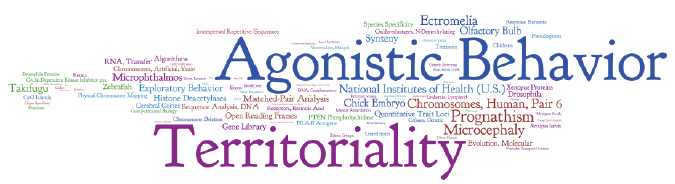
\includegraphics{nuagepoint}
\caption{exemple d'un nuage de mot}
\end{figure}


Chaque mot sera classé en fonction de son nombre d'ocurence dans les \textit{PMIDs}


\subsection{Recherche}
Un point important est la thématique recherchée. En effet, comme vu précédemment, les sujets d'articles englobent un grand nombre de thématique (génétique, maladies, chimie etc...) et donc le contexte peut changer pour des mêmes mots ou combinaisons de mots.
\section{Détection de transcription}

\subsection{Les facteurs de transcription}
Le facteur de transcription est une proteine qui a pour but lire et transcrire l'ADN.\\
Pour cela, elle parcours le brin d'ADN jusqu'à trouver le site dont la forme des nucléotides lui correspond.

\subsection{JASPAR 2014}

JASPAR est la plus grande base de données en open source de nucleotides stoqué sous forme de matrice décrivant la liaison de facteurs de transcription sur plusieurs espèces.

\subsection{ChIP-Seq}

ChIP-Seq = Chromatin ImmunoPrecipitation Sequencing\\
C'est une méthode utilisée pour analyser les interactions entre les protéines et l’ADN.\\
Cette technologie combine l’immunoprécipitation de la chromatine (ChIP), en utilisant des anticorps spécifiques d’une protéine d’intérêt et le séquençage haut débit.\\
Le principe consiste à fixer de façon covalente les protéines liées à l’ADN par un traitement chimique, de fragmenter la chromatine, d’immunoprécipiter les fragments en présence de l’anticorps d’intérêt et après purification et élimination des protéines, de séquencer les fragments d’ADN obtenus.\\
Il est ainsi possible de cartographier tous les sites de liaison sur l’ADN de cette protéine à l’échelle du génome.

\subsection{Les Zingers}

Lorsque l'on utilise les ChIP-Seq pour transcrire un brin d'ADN, nous repérons plus facilement les motifs au milieu du bruit comme on le voit sur le motif Hnf4a ci-dessous.\\

\begin{figure}{l}{}
\centering
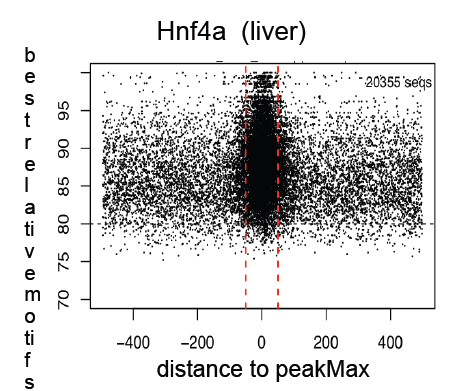
\includegraphics[scale=0.5]{peakmax}
\caption{Motif Hnf4a au milieu du bruit}
\end{figure}

Mais certain motifs apparaissent toujours peut importe la méthode utiliser sans que l'on comprennent réellement ce qu'il font là.\\
Ces motifs sont appelés ``Zingers''.

\section{Site de liaison d'allèle spécifique}
Dans cette partie sera présenté une manière plus affiné de détecter les sites de liaisons. 
\subsection{Définition}
Pour commencer un transcription, une protéïne est nécessaire. Celle-ci doit se fixer sur l'hélice. Une liaison d'allèle spécifique est ce même phénomène mais avec une protéine qui se liera d'avantages sur les allèles récessives.

\subsection{allèles préférées}

Une des premières observations faites est que sur les individus hétérozygotes (ayant deux allèles différentes) on remarque que certaines allèlles créent plus de sites de connections que une autre, alors que il était possible de s'attendre à une distribution equi-probable. 
\newline
\newline
Mais comme les allèles fortes s'expriment plus que les allèles récessives celà peut être dû à plusieurs raisons mais la plus commune est que, par selection naturelle, un gène subira une mutation, et aura un nombre supérieur de site de transcriptions que le précédent et ainsi pourra se transmettre plus facilement de génération en génération. De ce fait l'étude à de meilleurs chances de résultats si il est éffectué sur des gènes forts.
\begin{figure}{l}{}
\centering
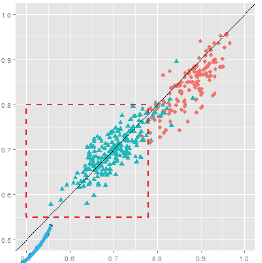
\includegraphics{grapheBestAllele}
\newline
\color{blue}
$\triangle$
\color{black} Allèles récessives
\\
\color{red}
$\Box$
\color{black} Allèles fortes
\caption{Allèle score}
\end{figure}


Pour trouver les places de liaisons de transcription, une unité a été crée: \textbf{PWM}: La matrice de position de poids.\\
Il s'agit d'une matrice où sont marquées les probabilités de chaque nucléotide d'apparaitre dans le site de liaison pour la transcription, ainsi que sa position.
\newline
\newline
Ceci a une importance particulière car grâce à ces matrices, il a été possible de remarquer que les liaisons ce faisaient plus sur les allèles récessives que les autres.
\newline
Mais ces travaux sont ralentis par le fait qu'il peut exister de multiples facteurs qui modifient le taux de transcription d'un site comme les mutations, l'hérédité et l'epigenetique.
\subsection{Recheche de site de liaison pour la transcription pour les lymphomes}

C'est ici que la présentation recoupe avec les travaux du Dr. Wasserman.
\newline
En effet, grâce aux outils présentés précédemment, beaucoup de données ont été recueillis, notamment des échantillons d'ADN, d'ARN de malades atteints de lymphomes.
\newline
\newline
Ensuite certaines zones du génomes ont été ciblés, et une des premières remarques est que les sites de transcriptions ont eu des taux de mutations plus élevé comparés aux séquences saines.
\newline
\newline
La mort des cellules, à un rôle dans ce fonctionnement. En effet, la mort des cellules est régulé d'une manière naturel et saine mais si cette régulation est perturbée celà peut causer des problèmes, dans le cas d'une diminution et dans le cas d'une augmentation un lymphome, par exemple. Une augmentation des cellules (ou plutôt une non décroissance normale du nombre de cellules) augmentent le nombre de site de liaison augmente. 



\section{Finalité}


\begin{hspace}{1cm}
Comme
\end{hspace}
expliqué, les sites de transcriptions sont importants dans l'expression du génome. Des malades attendent des avancées médicales mais la technologie bloque sur le séquencage ADN.  La recherche est mobilisée. Malgré l'aspect financier, il existe des initiatives qui permettent de partager des résultats, des expériences et d'aider la recherche (MeSH). 
\newline

\begin{hspace}{1cm}
Mais
\end{hspace} malgré cela la recherche bloque sur le séquencage du génome, pour se subsituer à cet obstacle de nouvelles idées émergent et au lieu de faire une recherche brute, des méthodes plus affinées sont implémentés par le Dr. Wasserman et dans le cas où le problème ne serait pas entièrement génétique mais dans son expression, via les sites de transcriptions. 
\newline

\subsection{perspectives}





\iffalse 
\subsubsection{Heading on level 3 (subsubsection)}
Nulla consequat massa quis enim. Donec pede justo, fringilla vel, aliquet nec, vulputate eget, arcu. In enim justo, rhoncus ut, imperdiet a, venenatis vitae, justo. Nullam dictum felis eu pede mollis pretium. Integer tincidunt. Cras dapibus. Vivamus elementum semper nisi. Aenean vulputate eleifend tellus. Aenean leo ligula, porttitor eu, consequat vitae, eleifend ac, enim.

\paragraph{Heading on level 4 (paragraph)}
Lorem ipsum dolor sit amet, consectetuer adipiscing elit. Aenean commodo ligula eget dolor. Aenean massa. Cum sociis natoque penatibus et magnis dis parturient montes, nascetur ridiculus mus. Donec quam felis, ultricies nec, pellentesque eu, pretium quis, sem. Nulla consequat massa quis enim. 


\section{Lists}
\subsection{Example for list (itemize)}
\begin{itemize}
	\item First item in a list 
	\item Second item in a list 
	\item Third item in a list
\end{itemize}

\subsubsection{Example for list (3*itemize)}
\begin{itemize}
	\item First item in a list 
		\begin{itemize}
		\item First item in a list 
			\begin{itemize}
			\item First item in a list 
			\item Second item in a list 
			\end{itemize}
		\item Second item in a list 
		\end{itemize}
	\item Second item in a list 
\end{itemize}

\subsection{Example for list (enumerate)}
\begin{enumerate}
	\item First item in a list 
	\item Second item in a list 
	\item Third item in a list
\end{enumerate}

\subsubsection{Example for list (3*enumerate)}
\begin{enumerate}
	\item First item in a list 
		\begin{enumerate}
		\item First item in a list 
			\begin{enumerate}
			\item First item in a list 
			\item Second item in a list 
			\end{enumerate}
		\item Second item in a list 
		\end{enumerate}
	\item Second item in a list 
\end{enumerate}

\section{Mathematics}
Let's display some math:
\begin{align} 
	\begin{split}
	(x+y)^3 	&= (x+y)^2(x+y)\\
					&=(x^2+2xy+y^2)(x+y)\\
					&=(x^3+2x^2y+xy^2) + (x^2y+2xy^2+y^3)\\
					&=x^3+3x^2y+3xy^2+y^3
	\end{split}					
\end{align}

\begin{align}
	A = 
	\begin{bmatrix}
	A_{11} & A_{21} \\
  	A_{21} & A_{22}
	\end{bmatrix}
\end{align}
\fi

\end{document}